\documentclass{report}
\usepackage{listings}
\usepackage{hyperref}
\usepackage{graphicx}
\graphicspath{ {./} }
\title{Computer Programming Homework 0}

\author{Sheng-Yi Hong}

\date{\today}

\begin{document}

\maketitle

\tableofcontents

\chapter{Requirement}

I recommend to use any Unix-Like OS (e.g. FreeBSD, MacOS, Linux) to finish this
homework. In windows, you can use either Virtual Machine or WSL to install Linux over Windows.

This homework require \textbf{google test} package. Google test is a unit test
library on C/C++. It helps us build test system over
er this homework so that you can check
if you write the correct code. It is avaliable on most of the operating system.
If you use Ubuntu Linux, you can use command \textbf{sudo apt install
  libgtest-dev -y} to install \textbf{google test} package. Other system you need to find by yourself.

\chapter{Review of C}

\section{Problem 1: Linked List}

Linked list is widely used in operating system kernel due to the high
performance on insert and delete elements compare with other data structure like
array. Linked list can be implemented from pointer which we have learned in
Computer Programming - I.

\subsection{Requirement}

In this problem, I want you to implement Linked List of \textbf{int32\_t} in C by
using array. Because you havn't learn structure, I want you to use array to
emulate the linking relationship. You have to modify all of the functions in \textbf{list.c} to
comply with the requirement. There are many types of Linked List. In this
problem I use the definition in C++
\href{https://en.cppreference.com/w/cpp/container/list}{std::list}. Not all of
the function in \textbf{std::list} is required. You only have to finish ones in
\textbf{list.c}. Of course, you can add some auxilary function to help you
implement linked list.

After finishing the requirement, you can run \textbf{make test} to test all of
your codes.
After passing all of the tests, you finish this problem.

\section{Problem 2: FSM}

I think you have learned Function in CP-I. Also, you have learned Pointer. A
pointer is a variable point to some memory address.
Surprisingly, the function also has its address. So pointer can also point to a
function.
To understand how to use function pointer, you can take a look to this website
\href{https://chenhh.gitbooks.io/parallel_processing/content/cython/function_pointer.html}{website}.

\subsection{Requirement}

Function pointer helps us solve many problems. In this problem, I want you to implement a
\href{https://zh.wikipedia.org/zh-tw/%E6%9C%89%E9%99%90%E7%8A%B6%E6%80%81%E6%9C%BA}{FSM
  ( Finite State Machine )} where each node is a function pointer.
We have to provide one function called \textbf{init()} and several functions for
nodes in this problem, which will return a function pointer of the initial node. The prototype of node function
\textbf{'void *(int)'} has an alias called \textbf{f\_type} in
\textbf{fsm.h}. This function prototype requires an index to indicate the next
node you want to jump and the return
value is the pointer to the next function. Why the return value is \textbf{void *}
instead of \textbf{f\_type} is due to the limitation of \textbf{typedef} in C.
We need to do type conversion manually after calling \textbf{f\_type} object.
Besides the return value, you are also required to print some information show
in the middle of node in the under graph(e.g. INIT, BBBB) on the
screen when executing the function in each node. When the index passed to the
function is not exist. You should return the pointer to the current node.
The following graph is the relationship(Arrow), index(First line in the circle),
and print string required(Second line in the circle). After
finishing, also run \textbf{make test} to test your code. If the string \textbf{OK} output,
your code is correct.


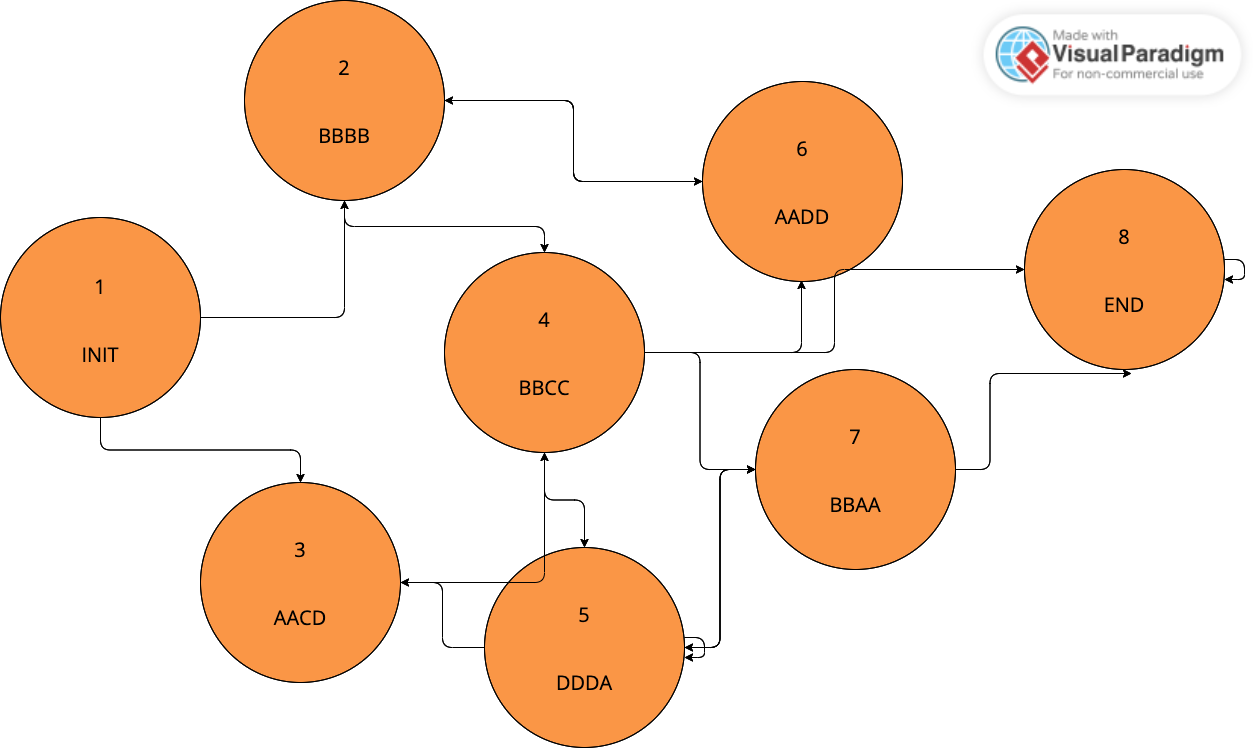
\includegraphics[scale=0.23]{graph}









\chapter{Preview of C++}

\section{Problem 3}

\section{Problem 4}

\end{document}